\documentclass[a4paper,12pt]{jsreport}
\usepackage{bm}
\usepackage[dvipdfmx]{graphicx}
\usepackage{ascmac}
\usepackage{amsthm}
\usepackage{amsmath, amssymb}
\theoremstyle{definition}
\newtheorem{theorem}{定理}
\newtheorem{definition}[theorem]{定義}
\newtheorem{prop}{命題}

\title{強化学習による最適観光ルート推定の研究}
\author{統計ファイナンス研究室\\
山口真哉\\
学籍番号:1116179036}
\date{2020年吉日}

\begin{document}
\maketitle
\tableofcontents

\chapter{はじめに}

最初はイントロ的なことを書く。
\section{現状と問題点}

最近の現状と問題点とか。

\section{解決策の提案}

こうしたらいい,とか。

\section{数式の書き方}

アインシュタイン方程式は以下の通りである。
\begin{equation}
    R_{\mu\nu} - \frac{1}{2} g_{\mu\nu} R = 
    \frac{8\pi G}{c^2} T_{\mu\nu}
\end{equation}

\chapter{グラフ理論}
この章の内容は、渡邊先生の離散数学の授業を元に記録した講義ノートの定義を使う.
\section{定義}
\begin{definition}[無向グラフ]
    有限集合$V=\{v_1,v_2,\ldots,v_n\}$と有限集合$E=\{e_1,e_2,\ldots,e_n\}\subset V^2$を考える.このとき,2つの集合の組$G=(V,E)$を無向グラフという.集合$V$の要素をグラフ$G$の頂点,集合$E$の要素を$G$の辺という.また,$e=\{u,v\}\in E$であるとき,$u$と$v$は隣接するという.
\end{definition}
\begin{definition}[部分グラフ]
    無向グラフ$G=(V,E),G'=(V',E')$について,$V\subset V',E\subset E'$であるとき, $G$は$G'$の部分グラフという.
\end{definition}
\begin{definition}[道,\ path]
    無向グラフ$G=(V,E)$,$G$の互いに異なる頂点列$P=(v_1,v_2,\ldots, v_{k+1})$とする.
    \begin{equation}
        V'=\{v_i|\ i=1,2,\ldots,k+1\}
    \end{equation}
    \begin{equation}
        E'=\{\{v_i,v_{i+1}\}\in E\ |\ i=1,2,\ldots,k\}
    \end{equation}
    としたとき$G'=(V',E')$を$G$の長さ$k$の道(path)という.特に,$s=v_1,\ t=v_{k+1}$とすると,$G'$を$s-t$ pathという.
\end{definition}
\begin{definition}[辺次数]
    $G=(V,E)$を無向グラフとする.そのとき,$v\in V$に対して,$v$に隣接する辺の集合を$\delta(v)$で表す.このとき,$\deg_G(v)=|\delta(v)|$を頂点$ v$の辺次数と呼ぶ.
\end{definition}
\section{グラフの表現}
$G=(V,E)$を無向グラフ,$n=|V|$とする.$w:E\to \mathbb{R}$を重み関数とする.$n$次正方行列$A=A(G)=a_{ij}$を
\begin{eqnarray}
    a_{ij}=
    \begin{cases}
        & w(e)\ (e=\{v_i,v_j\}\in E)\\
        & \infty\ \ \ \ ({\rm otherwise})
    \end{cases}
\end{eqnarray}
で定義し$A(G)$を無向グラフの隣接行列という.\\
隣接行列でグラフを表現する場合,2頂点間に辺があるか否かが定数時間で判定できるが,常に$O(|V|^2)$のメモリを消費する.道のように辺の数が少ない疎グラフの場合,隣接行列のほとんどが$\infty$で埋まることになる.\\ \\
集合の列$A=A(G)=a_v$を
\begin{equation}
    a_v=\{(u,w(e))\ |\ u\in V,\ e=\{u,v\}\in E \})
\end{equation}
とする.$A(G)$を隣接リストという.\\
このとき$O(|V|+|E|)$のメモリしか消費しない.



\chapter{強化学習}
学習に用いた強化学習の理論を記す.\\
環境とは行動と行動の応じた状態の変化が定義されており,ある状態への到達に対して報酬が与えられる空間のことである.強化学習では教師あり学習や教師なし学習とは異なり,データを与えるのではなく環境を与える.強化学習のモデル(agent)は状態を受け取り行動を出力する関数で,与えられた環境においてエピソード全体の報酬の総和を最大化するようにパラメータを調整する.
\section{強化学習の問題設定} 
強化学習において与えられた環境は「遷移先の状態は直前の状態とそこでの行動にのみ依存する.報酬は直前の状態と遷移先に依存する」ということを仮定する.この性質をマルコフ性と呼び,マルコフ性を持つ環境をマルコフ決定過程(MDP)と呼ぶ.MDPの構成要素は以下の4つである.\\
$s$ : 状態,$a$ : 行動,$T(s,a)$ : 状態遷移の確率,$R(s_t,s_{t+1})$ : 即時報酬\textbf{}
\begin{figure}[h]
    \centering
    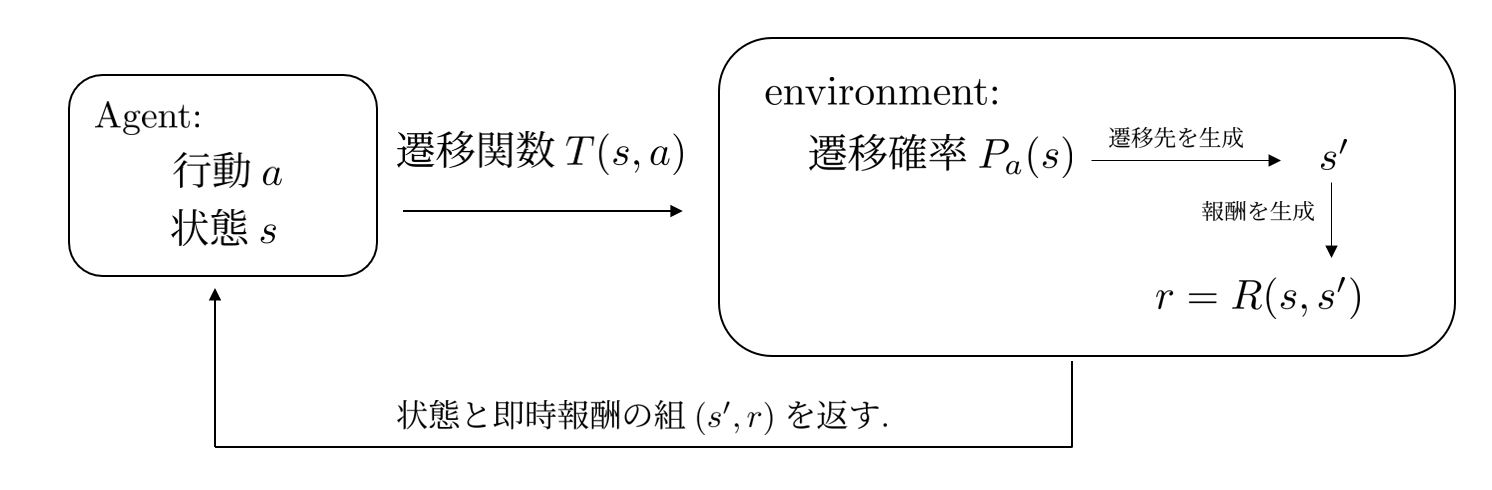
\includegraphics[width=10cm]{MDP.png}
    \caption{マルコフ決定過程の図式}
    \label{fig:MDP}
\end{figure}
\clearpage

MDPにおける報酬の総和は即時報酬の総和で定義される.エピソードの終了時刻を$T$としたとき,時刻$t$における報酬の総和$G_t$は以下のようになる.
\begin{equation}
    G_t:=\sum_{k=t+1}^Tr_t
\end{equation}

しかし実際には将来の即時報酬はわからないため,$G_t$はエピソード終了時でないと計算できない.エージェントが報酬の見積もりを立てる場合,割引率$\gamma\ (0\leq \gamma<1)$を用いて,
\begin{align}
    G_t&:=\sum_{k=t+1}^T \gamma^{t+1-k} r_k\\
    &=\sum_{k=0}^{T-t-1} \gamma^{k} r_{t+k+1}
\end{align}
と表し,期待報酬と呼ぶ.\\ 
強化学習では報酬の総和または期待報酬を最大化するようにエージェントの学習を行う.

\begin{prop}
    $G_t$は再帰性を持つ.
    つまり$0\leq t<T$において以下が成り立つ.
    \begin{equation}
        G_t=r_{t+1}+\gamma G_{t+1}
    \end{equation}
\end{prop}

\begin{proof}  
    \begin{align}
        G_t&=\sum_{k=t+1}^T \gamma^{t+1-k} r_k\\
        &=r_{t+1}+\gamma\sum_{k=t+2}^T \gamma^{t+1-k} r_k\\
        &=r_{t+1}+\gamma G_{t+1}
    \end{align}
\end{proof}

\section{価値の定義と算出}
前節で定義した価値$G_t$は報酬が必ず得られる賭して計算している.そのためagentの戦略(agentが状態を受け取り行動が出力される関数)の指標とするのには不適切である.\\
そこで戦略$\pi$,状態$s_t$における状態価値関数を以下で定義する.
\begin{equation}
    V_\pi(s_t):=\mathbb{E}[G_t\ |\ s_t=s]
\end{equation}
$G_t=r_{t+1}+\gamma G_{t+1}$より,
\begin{align}
    V_\pi(s_t)&=\mathbb{E}[G_t\ |\ s_t=s]\\
    &=\mathbb{E}[r_{t+1}+\gamma G_{t+1}\ |\ s_t=s]\\
    &=\mathbb{E}[r_{t+1}\ |\ s_t=s]+\gamma\mathbb{E}[G_{t+1}\ |\ s_t=s]\\
    &=\mathbb{E}[r_{t+1}\ |\ s_t=s]+\gamma V_\pi (s_{t+1})\\
\end{align}
行動確率$\pi(a|s)$,遷移確率$T(s'|s,a)$,報酬関数$R(s',s)$を用いて状態価値関数は以下のように表せる.
\begin{equation}
    V_\pi(s)=\sum_a\pi(a|s)\sum_{s'}T(s'|s,a)(R(s,s')+\gamma V_\pi(s'))
\end{equation}
この方程式をベルマン方程式という.\\
agentが常に価値が最大になるように行動を選択する場合以下が成り立つ.
\begin{equation}
    V(s)=\max_a\sum_{s'}T(s'|s,a)(R(s,s')+\gamma V(s'))
\end{equation}
特に報酬が状態にのみで決まるとき以下が成立.
\begin{equation}
    V(s)=R(s)+\gamma\max_a\sum_{s'}T(s'|s,a)V(s')
\end{equation}
状態価値関数$V$は価値の評価や更新に使われる.
戦略で行動を決定し, その評価, 更新に行動評価が使われる.\\
実際の学習では,更新差異が小さな値$\varepsilon$未満になるまでベルマン方程式の解を複数回繰り返して値の精度を高めていく.
\begin{equation}
    V(s)\leftarrow\max_a\sum_{s'}T(s'|s,a)(R(s,s')+\gamma V(s'))
\end{equation}
これを価値反復法という.
\section{学習}





\chapter{巡回セールスマン問題}
巡回セールスマン問題とは,\ 頂点数$N$の重み付き有向グラフの隣接行列$D$が与えられる.\ 頂点$s$から頂点$t$への道の集合の中で重みの総和が最小の道を求める問題である.
\section{道の全列挙}
始点$s$と終点$t$を除く集合を$X=\{1,2\ldots ,n\}\setminus\{s,t\}$,$n$次対称群を$S_n$とする.
\begin{eqnarray}
    \min_{\sigma\in S_{N-2}}
    \left(D_{s,\sigma(X_0)} + D_{\sigma(X_{n-2}),t} +
    \sum_{i=1}^{n-3}
        D_{\sigma(X_i),\sigma(X_{i+1})} 
    \right)
\end{eqnarray}
とすると,$|S_{N-2}|=(N-2)!$なので,\\ 巡回セールスマン問題を時間計算量$O((N-1)!)$で求めることができる.

\section{集合に対する動的計画法}
$S$を既に訪れた頂点集合,現在頂点$v$にいるとする.
$$dp(S,v)=(vに来るまでにかかる距離の総和の最小値)$$
このとき,以下の漸化式が成立.
\begin{eqnarray}
    \begin{cases}
        & dp(\{s\},s)=0\\
        & dp(S,v)=\min_{u \notin S}dp(S\setminus\{u\},u)+dp(u,v)
    \end{cases}
\end{eqnarray}
$X=\{1,2\ldots ,n\}$としたとき,巡回セールスマン問題の解は$dp(X,t)$である.\\
よって時間計算量$O(2^NN^2)$で解くことができた.
\section{ヒューリスティックな解法}
集合に対する動的計画法を用いた解法は$N$が大きくなるにつれて指数的に時間計算量が大きくなるため,頂点数が大きな巡回セールスマン問題において計算結果を出すことができない.
例えば山登り法や焼きなまし法,遺伝的アルゴリズムを用いることにより多項式時間で近似解を求めることができる.
\chapter{main}









\chapter{}
データは参考文献\cite{rika} にあったものを使った.
この文献\cite{ten}も参考にした。


\chapter{最後に}

結論とか,まとめとか。
最後にいうのもなんだが,ベクトルの書き方。
\begin{itemize}
  \item 普通の$\alpha$は\verb|\alpha|で書く。
  \item \verb|$\vec{\alpha}$| で $\vec{\alpha}$
  \item \verb|\usepackage{bm}| している場合は
        \verb|$\bm{\alpha}$| で $\bm{\alpha}$
  \item 並べると,$\alpha$, $\vec{\alpha}$, $\bm{\alpha}$
\end{itemize}


\chapter*{謝辞}

謝辞には第何章とかの番号をつけなくてもよいので,そんなときは,
\verb|\chapter*{ }| という具合に書きます。

みなさん,ありがとう.(普通の人が見るのは,イントロと謝辞だけ... 
という説もあるから,忘れないで書く.)

\appendix
\chapter{付録があるときは}
プログラム文とかを書いてページ数を稼ぎたいときは,
以下のようにしてみます。

\begin{verbatim}
#include <iostream>
using namespace std;
int main() {  
    for(int i = 1; i <= 5; i++) {
        cout << "こんにちは, C++ の世界!   "  << i << endl;
    }
    return 0;
}
\end{verbatim}
\verb|\usepackage{ascmac}|して\verb|screen| 環境を使うと,枠がつきます。
\begin{screen}
\begin{verbatim}
#include <iostream>
using namespace std;
int main() {  
    for(int i = 1; i <= 5; i++) {
        cout << "こんにちは, C++ の世界!   "  << i << endl;
    }
    return 0;
}
\end{verbatim}
\end{screen}

\begin{thebibliography}{99}
\bibitem{rika} 国立天文台編,理科年表 (丸善)
\bibitem{ten} 天文年鑑,誠文堂新光社。
\end{thebibliography}

\end{document}